\documentclass[aspectratio=169]{beamer}
% Add slides directory to search path for Dartmouth theme
\makeatletter
\def\input@path{{../}}
\makeatother
\usetheme{Dartmouth}
\usepackage{graphicx}
\usepackage{tikz}
\usetikzlibrary{shapes.geometric, arrows.meta, positioning, fit, backgrounds}
\usepackage{pgfplots}
\pgfplotsset{compat=1.18}
\usepackage{amsmath}
\usepackage{listings}
\usepackage{xcolor}
\usepackage{booktabs}
\usepackage{hyperref}
\usepackage{tcolorbox}

% Color scheme
\definecolor{darkblue}{RGB}{0,82,155}
\definecolor{lightblue}{RGB}{100,181,246}
\definecolor{darkgreen}{RGB}{46,125,50}
\definecolor{orange}{RGB}{255,152,0}
\definecolor{purple}{RGB}{156,39,176}
\definecolor{teal}{RGB}{0,150,136}

\setbeamercolor{frametitle}{bg=darkblue}
\setbeamercolor{progress bar}{fg=lightblue,bg=lightblue!30}

% Code listing settings
\lstset{
    basicstyle=\ttfamily\small,
    breaklines=true,
    frame=single,
    backgroundcolor=\color{gray!10},
    keywordstyle=\color{darkblue}\bfseries,
    commentstyle=\color{darkgreen}\itshape,
    stringstyle=\color{orange},
    showstringspaces=false,
    language=Python,
    numbers=left,
    numberstyle=\tiny\color{gray}
}

% Custom boxes
\newtcolorbox{discussionbox}{
    colback=lightblue!10,
    colframe=darkblue,
    title=💬 Discussion Question,
    fonttitle=\bfseries
}

\newtcolorbox{thinkbox}{
    colback=orange!10,
    colframe=orange,
    title=💭 Think About It,
    fonttitle=\bfseries
}

\newtcolorbox{futurebox}{
    colback=purple!10,
    colframe=purple,
    title=🔮 Future Directions,
    fonttitle=\bfseries
}

\title{Week 9: RAG \& Mixture of Experts}
\subtitle{Enhancing LLMs with Retrieval and Routing 🔍🚀}
\author{PSYC 51.07: Models of Language and Communication}
\date{}

\begin{document}

% ============================================================
% TITLE SLIDE
% ============================================================
\begin{frame}[shrink=10]
\titlepage
\end{frame}

% ============================================================
% OVERVIEW
% ============================================================
\begin{frame}[shrink=10]{Today's Journey 🗺️}
\large
\begin{enumerate}\setlength{\itemsep}{0pt}
    \item 🔍 \textbf{Retrieval Augmented Generation (RAG)}: Grounding LLMs in external knowledge
    \item 🎯 \textbf{Mixture of Experts (MoE)}: Efficient scaling through specialization
    \item 📊 \textbf{Self-Supervised Learning}: SimCLR and contrastive methods
    \item 🖼️ \textbf{Multimodal Learning}: CLIP and vision-language alignment
    \item 🔮 \textbf{What's Next for LLMs?}: Future directions and open problems
    \item 🎓 \textbf{Final Project}: Guidelines and inspiration
\end{enumerate}

\vspace{1em}
\begin{center}
\textit{Goal: Look toward the future while grounding ourselves in current techniques}
\end{center}
\end{frame}

% ============================================================
% SECTION 1: RAG
% ============================================================
\section{Retrieval Augmented Generation}

\begin{frame}[shrink=10]{The Limits of Parametric Memory 🧠}
\begin{discussionbox}
\textbf{What are the limits of parametric memory?}

Consider: An LLM's knowledge is frozen at training time...
\end{discussionbox}

\vspace{0.5em}

\textbf{Problems with purely parametric models:}
\begin{itemize}\setlength{\itemsep}{0pt}
    \item ❌ \textbf{Knowledge cutoff}: No information after training
    \item ❌ \textbf{Hallucinations}: Models confidently generate false information
    \item ❌ \textbf{No source attribution}: Can't cite where information comes from
    \item ❌ \textbf{Expensive updates}: Retraining for new information is costly
    \item ❌ \textbf{Privacy concerns}: Sensitive data baked into parameters
    \item ❌ \textbf{Domain specificity}: Limited knowledge of specialized domains
\end{itemize}

\vspace{0.5em}
\textbf{Solution:} Combine parametric knowledge with non-parametric retrieval! 🔍
\end{frame}

\begin{frame}[shrink=10]{What is RAG? 📚}
\begin{block}{Retrieval Augmented Generation}
A technique that enhances LLMs by retrieving relevant documents from an external knowledge base and using them to inform generation.
\end{block}

\vspace{1em}

\textbf{Key Idea:} Instead of relying only on learned parameters, the model can "look things up"!

\vspace{1em}

\begin{columns}[T]
\begin{column}{0.45\textwidth}
\textbf{Traditional LLM:}
\begin{itemize}\setlength{\itemsep}{0pt}
    \item Question → Model → Answer
    \item Only parametric knowledge
    \item Fixed at training time
\end{itemize}
\end{column}

\begin{column}{0.45\textwidth}
\textbf{RAG Pipeline:}
\begin{itemize}\setlength{\itemsep}{0pt}
    \item Question → Retrieve Docs
    \item Docs + Question → Model
    \item Grounded Answer
\end{itemize}
\end{column}
\end{columns}

\vspace{1em}
\small
\textit{Reference: Lewis et al. (2020) - "Retrieval-Augmented Generation for Knowledge-Intensive NLP Tasks"}
\end{frame}

\begin{frame}[shrink=5]{RAG Architecture 🏗️}
\begin{center}
\begin{tikzpicture}[scale=0.85][
    node distance=1.5cm,
    box/.style={rectangle, rounded corners, draw, fill=blue!20, text width=2.5cm, align=center, minimum height=1cm},
    databox/.style={rectangle, draw, fill=green!20, text width=2.5cm, align=center, minimum height=1cm},
    arrow/.style={-{Stealth[length=3mm]}, thick}
]

% User query
\node[databox] (query) {User Query\\"What is RAG?"};

% Embedding
\node[box, right=of query] (embed) {Embedding Model};

% Vector DB
\node[databox, above right=0.5cm and 1cm of embed] (vectordb) {Vector Database\\(Embeddings)};

% Retrieved docs
\node[databox, below right=0.5cm and 1cm of embed] (docs) {Retrieved\\Documents};

% Retrieval
\node[box, right=3cm of embed] (retrieve) {Similarity\\Search};

% Augmented prompt
\node[databox, right=of retrieve] (prompt) {Augmented\\Prompt};

% LLM
\node[box, right=of prompt] (llm) {LLM\\Generation};

% Response
\node[databox, right=of llm] (response) {Grounded\\Response};

% Arrows
\draw[arrow] (query) -- (embed);
\draw[arrow] (embed) -- (retrieve);
\draw[arrow] (vectordb) -- (retrieve);
\draw[arrow] (retrieve) -- (docs);
\draw[arrow] (docs) -- (prompt);
\draw[arrow] (query.east) -- ++(0.5,0) |- (prompt.west);
\draw[arrow] (prompt) -- (llm);
\draw[arrow] (llm) -- (response);

\end{tikzpicture}
\end{center}

\vspace{0.5em}
\textbf{Steps:}
\begin{enumerate}\setlength{\itemsep}{0pt}
    \item Embed user query
    \item Search vector database for similar documents
    \item Retrieve top-k most relevant documents
    \item Augment prompt with retrieved context
    \item Generate answer using LLM
\end{enumerate}
\end{frame}

\begin{frame}[fragile]{RAG Implementation Example 💻}
\textbf{Basic RAG with HuggingFace and ChromaDB:}

\begin{lstlisting}[language=Python, basicstyle=\ttfamily\tiny]
from langchain.vectorstores import Chroma
from langchain.embeddings import HuggingFaceEmbeddings
from langchain.llms import HuggingFacePipeline
from langchain.chains import RetrievalQA

# 1. Create vector database from documents
embeddings = HuggingFaceEmbeddings(model_name="sentence-transformers/all-MiniLM-L6-v2")
vectordb = Chroma.from_documents(
    documents=docs,
    embedding=embeddings,
    persist_directory="./chroma_db"
)

# 2. Set up retriever
retriever = vectordb.as_retriever(
    search_type="similarity",
    search_kwargs={"k": 3}  # Retrieve top 3 documents
)

# 3. Create RAG chain
llm = HuggingFacePipeline.from_model_id(
    model_id="meta-llama/Llama-2-7b-chat-hf",
    task="text-generation"
)

qa_chain = RetrievalQA.from_chain_type(
    llm=llm,
    retriever=retriever,
    return_source_documents=True
)

# 4. Query
result = qa_chain({"query": "What is retrieval augmented generation?"})
print(result['result'])
print("\nSources:", result['source_documents'])
\end{lstlisting}

\small
\textit{Tutorial: HuggingFace Advanced RAG - \url{https://huggingface.co/learn/cookbook/advanced_rag}}
\end{frame}

\begin{frame}[shrink=10]{Advanced RAG Techniques 🚀}
\begin{columns}[T]
\begin{column}{0.48\textwidth}
\textbf{Self-RAG} (Asai et al., 2023)
\begin{itemize}\setlength{\itemsep}{0pt}
    \item Model decides \textit{when} to retrieve
    \item Self-reflects on retrieval quality
    \item Critique and refine generations
    \item More adaptive and efficient
\end{itemize}

\vspace{1em}

\textbf{Key Idea:}
Not every query needs retrieval!
\end{column}

\begin{column}{0.48\textwidth}
\textbf{Corrective RAG} (Yan et al., 2024)
\begin{itemize}\setlength{\itemsep}{0pt}
    \item Evaluates retrieved documents
    \item Filters irrelevant content
    \item Re-retrieves if needed
    \item Decomposes complex queries
\end{itemize}

\vspace{1em}

\textbf{Key Idea:}
Quality over quantity in retrieval!
\end{column}
\end{columns}

\vspace{1em}

\begin{alertblock}{Evolution of RAG}
\textbf{Basic RAG} → \textbf{Self-RAG} → \textbf{Corrective RAG} → \textbf{Agentic RAG}

The field is moving toward more autonomous, self-correcting systems!
\end{alertblock}

\small
\textit{References: Asai et al. (2023) - Self-RAG; Yan et al. (2024) - Corrective RAG}
\end{frame}

\begin{frame}[shrink=10]{RAG Components Deep Dive 🔬}
\begin{enumerate}\setlength{\itemsep}{0pt}
    \item \textbf{Document Processing}
    \begin{itemize}\setlength{\itemsep}{0pt}
        \item Chunking strategies (fixed, semantic, recursive)
        \item Metadata extraction
        \item Deduplication
    \end{itemize}

    \vspace{0.3em}

    \item \textbf{Embedding Models}
    \begin{itemize}\setlength{\itemsep}{0pt}
        \item Dense retrieval: Sentence-BERT, E5, BGE
        \item Sparse retrieval: BM25, TF-IDF
        \item Hybrid approaches
    \end{itemize}

    \vspace{0.3em}

    \item \textbf{Vector Databases}
    \begin{itemize}\setlength{\itemsep}{0pt}
        \item FAISS, ChromaDB, Pinecone, Weaviate, Qdrant
        \item Indexing strategies (IVF, HNSW)
        \item Approximate nearest neighbor search
    \end{itemize}

    \vspace{0.3em}

    \item \textbf{Prompt Engineering}
    \begin{itemize}\setlength{\itemsep}{0pt}
        \item How to format retrieved context
        \item Instruction templates
        \item Source attribution
    \end{itemize}
\end{enumerate}
\end{frame}

\begin{frame}{Comparing RAG Approaches 📊}
\begin{table}
\small
\begin{tabular}{l p{3cm} p{3cm} p{3.5cm}}
\toprule
\textbf{Approach} & \textbf{When to Retrieve} & \textbf{How to Filter} & \textbf{Best For} \\
\midrule
\textbf{Naive RAG} & Always & Top-k similarity & Simple Q\&A, prototyping \\
\addlinespace
\textbf{Self-RAG} & Model decides & Self-reflection tokens & Adaptive retrieval needs \\
\addlinespace
\textbf{Corrective RAG} & Always & Relevance scoring & High-precision requirements \\
\addlinespace
\textbf{HyDE} & Always (on generated answer) & Similarity to hypothesis & Complex reasoning \\
\addlinespace
\textbf{Agentic RAG} & Tool-based decision & Multi-step filtering & Complex workflows \\
\bottomrule
\end{tabular}
\end{table}

\vspace{1em}

\begin{thinkbox}
\textbf{Trade-offs:} Simplicity vs. Performance vs. Latency vs. Cost

What's the right balance for your use case?
\end{thinkbox}
\end{frame}

\begin{frame}[shrink=10]{RAG in Production 🏭}
\textbf{Real-world considerations:}

\begin{columns}[T]
\begin{column}{0.48\textwidth}
\textbf{Challenges:}
\begin{itemize}\setlength{\itemsep}{0pt}
    \item 💰 Cost: Embedding + storage + inference
    \item ⚡ Latency: Retrieval adds overhead
    \item 📏 Context window limits
    \item 🎯 Retrieval quality issues
    \item 🔄 Keeping data fresh
    \item 🔒 Security and privacy
\end{itemize}
\end{column}

\begin{column}{0.48\textwidth}
\textbf{Solutions:}
\begin{itemize}\setlength{\itemsep}{0pt}
    \item Caching embeddings
    \item Semantic caching
    \item Incremental indexing
    \item Re-ranking strategies
    \item Smaller, efficient models
    \item Hybrid search methods
\end{itemize}
\end{column}
\end{columns}

\vspace{1em}

\begin{alertblock}{Production Tip}
Start simple (Naive RAG), measure performance, then optimize based on actual bottlenecks!
\end{alertblock}

\small
\textit{Resource: HuggingFace Agents Course - \url{https://huggingface.co/learn/agents-course}}
\end{frame}

% ============================================================
% SECTION 2: MIXTURE OF EXPERTS
% ============================================================
\section{Mixture of Experts}

\begin{frame}{The Scaling Challenge 📈}
\begin{discussionbox}
Larger models are better... but training 100B+ parameter models is:
\begin{itemize}\setlength{\itemsep}{0pt}
    \item Computationally expensive 💸
    \item Energy intensive 🔥
    \item Slow to train ⏳
    \item Slow at inference 🐌
\end{itemize}

Can we get the benefits of scale without the costs?
\end{discussionbox}

\vspace{1em}

\textbf{Key Insight:} Not all parameters need to be active for every input!

\vspace{0.5em}

\begin{block}{Mixture of Experts (MoE)}
A neural network architecture where different "expert" sub-networks specialize in different parts of the input space, with a gating mechanism that routes inputs to the appropriate experts.
\end{block}

\small
\textit{Reference: Shazeer et al. (2017) - "Outrageously Large Neural Networks: The Sparsely-Gated Mixture-of-Experts Layer"}
\end{frame}

\begin{frame}[shrink=5]{MoE Architecture 🏗️}
\begin{center}
\begin{tikzpicture}[scale=0.85][
    node distance=1.2cm,
    expert/.style={rectangle, rounded corners, draw, fill=blue!30, minimum width=1.8cm, minimum height=0.8cm, align=center},
    router/.style={rectangle, rounded corners, draw, fill=orange!40, minimum width=2.5cm, minimum height=0.8cm, align=center},
    input/.style={circle, draw, fill=green!30, minimum size=0.8cm},
    output/.style={circle, draw, fill=purple!30, minimum size=0.8cm}
]

% Input
\node[input] (input) {$x$};

% Router
\node[router, above=of input] (router) {Router/Gate\\$g(x)$};

% Experts
\node[expert, above left=1cm and 1.5cm of router] (expert1) {Expert 1\\(Math)};
\node[expert, above=1.5cm of router] (expert2) {Expert 2\\(Code)};
\node[expert, above right=1cm and 1.5cm of router] (expert3) {Expert 3\\(Lang)};
\node[expert, right=3cm of expert3] (expertn) {Expert N\\(...)};

% Output aggregation
\node[output, above=2cm of router] (output) {$y$};

% Arrows from input to router
\draw[->, thick] (input) -- (router);

% Arrows from router to experts with weights
\draw[->, thick, blue] (router) -- (expert1) node[midway, left, font=\tiny] {$w_1=0.7$};
\draw[->, thick, blue] (router) -- (expert2) node[midway, left, font=\tiny] {$w_2=0.3$};
\draw[->, thick, gray, dashed] (router) -- (expert3) node[midway, right, font=\tiny] {$w_3=0.0$};
\draw[->, thick, gray, dashed] (router.east) -- ++(1.5,0) |- (expertn.west) node[near start, above, font=\tiny] {$w_n=0.0$};

% Arrows from experts to output
\draw[->, thick, blue] (expert1) |- (output);
\draw[->, thick, blue] (expert2) -- (output);
\draw[->, thick, gray, dashed] (expert3) |- (output);
\draw[->, thick, gray, dashed] (expertn) |- (output);

% Formula
\node[below=0.3cm of input, font=\footnotesize] {$y = \sum_{i=1}^{N} g(x)_i \cdot E_i(x)$};

\end{tikzpicture}
\end{center}

\vspace{0.5em}
\textbf{Key Components:}
\begin{itemize}\setlength{\itemsep}{0pt}
    \item \textbf{Experts}: Specialized feed-forward networks (typically only top-2 are active)
    \item \textbf{Router}: Learned gating function that assigns weights to experts
    \item \textbf{Sparse Activation}: Only a few experts process each token
\end{itemize}
\end{frame}

\begin{frame}[shrink=10]{How MoE Works: The Router 🎯}
\textbf{Routing Mechanism:}

\begin{enumerate}\setlength{\itemsep}{0pt}
    \item For input $x$, router computes scores: $h(x) = W_g \cdot x$
    \item Apply softmax to get probabilities: $g(x) = \text{softmax}(h(x))$
    \item Select top-$k$ experts (typically $k=2$)
    \item Route token only to selected experts
    \item Aggregate outputs: $y = \sum_{i \in \text{top-k}} g(x)_i \cdot E_i(x)$
\end{enumerate}

\vspace{1em}

\textbf{Benefits:}
\begin{itemize}\setlength{\itemsep}{0pt}
    \item ✅ \textbf{Sparse computation}: Only 2 out of N experts active
    \item ✅ \textbf{Scalable}: Can add more experts without increasing per-token cost
    \item ✅ \textbf{Specialization}: Experts learn different capabilities
    \item ✅ \textbf{Efficiency}: Better quality/compute ratio
\end{itemize}

\vspace{0.5em}

\begin{thinkbox}
\textbf{Analogy:} Like having specialized doctors (cardiologist, neurologist, etc.) instead of one general practitioner handling everything!
\end{thinkbox}
\end{frame}

\begin{frame}[shrink=10]{MoE Challenges \& Solutions ⚠️}
\begin{columns}[T]
\begin{column}{0.48\textwidth}
\textbf{Challenges:}
\begin{enumerate}\setlength{\itemsep}{0pt}
    \item \textbf{Load Balancing}
    \begin{itemize}\setlength{\itemsep}{0pt}
        \item Some experts overused
        \item Others underutilized
    \end{itemize}

    \vspace{0.3em}

    \item \textbf{Training Instability}
    \begin{itemize}\setlength{\itemsep}{0pt}
        \item Routing collapse
        \item Expert specialization
    \end{itemize}

    \vspace{0.3em}

    \item \textbf{Memory Requirements}
    \begin{itemize}\setlength{\itemsep}{0pt}
        \item All experts in memory
        \item High bandwidth needs
    \end{itemize}
\end{enumerate}
\end{column}

\begin{column}{0.48\textwidth}
\textbf{Solutions:}
\begin{enumerate}\setlength{\itemsep}{0pt}
    \item \textbf{Load Balancing Loss}
    \begin{itemize}\setlength{\itemsep}{0pt}
        \item Auxiliary loss term
        \item Encourages uniform usage
    \end{itemize}

    \vspace{0.3em}

    \item \textbf{Expert Capacity}
    \begin{itemize}\setlength{\itemsep}{0pt}
        \item Limit tokens per expert
        \item Dynamic capacity buffers
    \end{itemize}

    \vspace{0.3em}

    \item \textbf{Expert Parallelism}
    \begin{itemize}\setlength{\itemsep}{0pt}
        \item Distribute experts across GPUs
        \item Optimize communication
    \end{itemize}
\end{enumerate}
\end{column}
\end{columns}

\vspace{1em}

\begin{alertblock}{Key Innovation}
Load balancing loss: $\mathcal{L}_{\text{balance}} = \alpha \cdot \sum_{i=1}^{N} f_i \cdot P_i$

where $f_i$ is the fraction of tokens routed to expert $i$, and $P_i$ is its probability.
\end{alertblock}
\end{frame}

\begin{frame}{Mixtral 8x7B: MoE in Action 🎬}
\begin{block}{Mixtral 8x7B (Jiang et al., 2024)}
A state-of-the-art sparse mixture of experts model with 8 experts, each 7B parameters.
\end{block}

\vspace{0.5em}

\textbf{Architecture:}
\begin{itemize}\setlength{\itemsep}{0pt}
    \item \textbf{Total parameters}: 47B (8 experts × 7B, minus shared layers)
    \item \textbf{Active parameters}: 13B (only 2 experts active per token)
    \item \textbf{Performance}: Matches or exceeds Llama 2 70B
    \item \textbf{Speed}: 6× faster inference than dense 70B model
\end{itemize}

\vspace{0.5em}

\textbf{Key Results:}
\begin{table}
\tiny
\begin{tabular}{l c c c}
\toprule
\textbf{Model} & \textbf{Active Params} & \textbf{MMLU} & \textbf{Speed} \\
\midrule
Llama 2 70B & 70B & 69.7 & 1× \\
Mixtral 8x7B & 13B & 70.6 & 6× \\
\bottomrule
\end{tabular}
\end{table}

\vspace{0.5em}
\small
\textit{Reference: Jiang et al. (2024) - "Mixtral of Experts"}

\textit{Blog: \url{https://huggingface.co/blog/moe}}
\end{frame}

\begin{frame}[shrink=10]{MoE vs Dense Models 📊}
\begin{center}
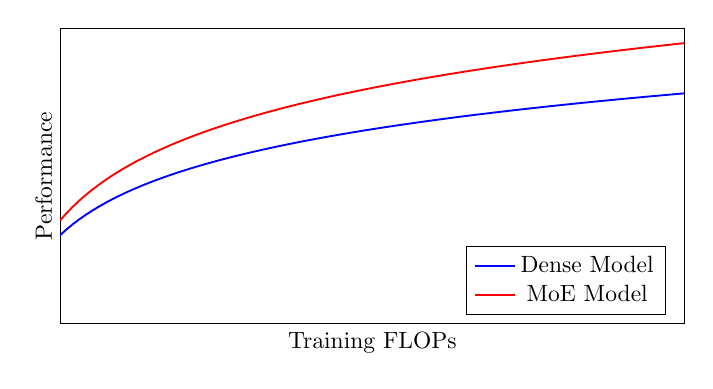
\begin{tikzpicture}[scale=0.85]
    \begin{axis}[
        width=0.9\textwidth,
        height=6cm,
        xlabel={Training FLOPs},
        ylabel={Performance},
        legend pos=south east,
        grid=major,
        xmin=0, xmax=10,
        ymin=0, ymax=10,
        xtick=\empty,
        ytick=\empty
    ]

    % Dense model curve
    \addplot[blue, thick, domain=0:10, samples=100] {2*ln(x+1) + 3};
    \addlegendentry{Dense Model}

    % MoE model curve (better efficiency)
    \addplot[red, thick, domain=0:10, samples=100] {2.5*ln(x+1) + 3.5};
    \addlegendentry{MoE Model}

    \end{axis}
\end{tikzpicture}
\end{center}

\textbf{Trade-offs:}
\begin{columns}[T]
\begin{column}{0.48\textwidth}
\textbf{MoE Advantages:}
\begin{itemize}\setlength{\itemsep}{0pt}
    \item Better compute efficiency
    \item Faster training
    \item Faster inference
    \item Modular specialization
\end{itemize}
\end{column}

\begin{column}{0.48\textwidth}
\textbf{Dense Advantages:}
\begin{itemize}\setlength{\itemsep}{0pt}
    \item Simpler architecture
    \item Easier to train
    \item Lower memory usage
    \item Better on small scale
\end{itemize}
\end{column}
\end{columns}
\end{frame}

% ============================================================
% SECTION 3: SELF-SUPERVISED LEARNING
% ============================================================
\section{Self-Supervised \& Contrastive Learning}

\begin{frame}[shrink=10]{Self-Supervised Learning 🔄}
\small
\begin{block}{Self-Supervised Learning}
Learning representations from unlabeled data by creating pretext tasks where the data itself provides the supervision signal.
\end{block}

\vspace{1em}

\textbf{Why is this important?}
\begin{itemize}\setlength{\itemsep}{0pt}
    \item Labeled data is expensive and scarce
    \item Unlabeled data is abundant
    \item Learn general-purpose representations
    \item Transfer to downstream tasks
\end{itemize}

\vspace{1em}

\textbf{Examples of pretext tasks:}
\begin{itemize}\setlength{\itemsep}{0pt}
    \item \textbf{Language}: Masked language modeling (BERT), next token prediction (GPT)
    \item \textbf{Vision}: Predicting rotations, colorization, jigsaw puzzles
    \item \textbf{Contrastive}: Making similar things close, dissimilar things far apart
\end{itemize}
\end{frame}

\begin{frame}[shrink=5]{Contrastive Learning 🎯}
\begin{center}
\textbf{Core Idea:} Learn by contrasting positive pairs against negative pairs

\vspace{1em}

\begin{tikzpicture}[scale=0.85][
    node distance=1.5cm,
    imgnode/.style={rectangle, draw, fill=blue!20, minimum size=1cm},
    anchornode/.style={rectangle, draw, fill=green!40, minimum size=1cm},
    posnode/.style={rectangle, draw, fill=green!20, minimum size=1cm},
    negnode/.style={rectangle, draw, fill=red!20, minimum size=1cm}
]

% Anchor
\node[anchornode] (anchor) {🐕};
\node[below=0.1cm of anchor, font=\tiny] {Anchor};

% Positive
\node[posnode, right=2cm of anchor] (pos) {🐕};
\node[below=0.1cm of pos, font=\tiny] {Positive};

% Negatives
\node[negnode, above right=0.5cm and 3.5cm of anchor] (neg1) {🐱};
\node[negnode, right=3.5cm of anchor] (neg2) {🚗};
\node[negnode, below right=0.5cm and 3.5cm of anchor] (neg3) {🌳};

% Arrows
\draw[->, thick, green!60!black] (anchor) -- (pos) node[midway, above, font=\footnotesize] {Pull together};
\draw[->, thick, red!60!black] (anchor) -- (neg1) node[midway, above, font=\tiny] {Push apart};
\draw[->, thick, red!60!black] (anchor) -- (neg2) node[midway, above, font=\tiny] {Push apart};
\draw[->, thick, red!60!black] (anchor) -- (neg3) node[midway, below, font=\tiny] {Push apart};

\end{tikzpicture}
\end{center}

\vspace{0.5em}

\textbf{Objective:} $\mathcal{L} = -\log \frac{\exp(\text{sim}(z_i, z_i^+) / \tau)}{\sum_{j=1}^{N} \exp(\text{sim}(z_i, z_j) / \tau)}$

where $z_i$ is anchor, $z_i^+$ is positive, and $\{z_j\}$ includes negatives.
\end{frame}

\begin{frame}[shrink=10]{SimCLR: Simple Contrastive Learning 🔬}
\begin{block}{SimCLR (Chen et al., 2020)}
"A Simple Framework for Contrastive Learning of Visual Representations"
\end{block}

\textbf{Method:}
\begin{enumerate}\setlength{\itemsep}{0pt}
    \item Take an image
    \item Apply two different random augmentations (crop, color, blur, etc.)
    \item Encode both views with a neural network
    \item Pull representations of the two views together
    \item Push apart from other images in the batch
\end{enumerate}

\vspace{0.5em}

\textbf{Key Innovations:}
\begin{itemize}\setlength{\itemsep}{0pt}
    \item Strong data augmentation is crucial
    \item Learnable projection head improves performance
    \item Large batch sizes help (more negatives)
    \item Longer training = better representations
\end{itemize}

\vspace{0.5em}

\textbf{Result:} Matches or exceeds supervised learning on ImageNet with only self-supervision!

\small
\textit{Reference: Chen et al. (2020) - "A Simple Framework for Contrastive Learning of Visual Representations"}
\end{frame}

\begin{frame}[shrink=5]{CLIP: Connecting Vision \& Language 🖼️📝}
\begin{block}{CLIP (Radford et al., 2021)}
"Learning Transferable Visual Models From Natural Language Supervision"
\end{block}

\textbf{Big Idea:} Train vision and language encoders together using contrastive learning!

\vspace{0.5em}

\begin{center}
\begin{tikzpicture}[scale=0.85][
    node distance=1cm,
    box/.style={rectangle, rounded corners, draw, fill=blue!20, minimum width=2cm, minimum height=0.8cm, align=center},
    encoder/.style={rectangle, rounded corners, draw, fill=orange!30, minimum width=2.5cm, minimum height=1.2cm, align=center}
]

% Images
\node[box] (img1) {🐕 Image 1};
\node[box, below=0.3cm of img1] (img2) {🐱 Image 2};
\node[box, below=0.3cm of img2] (img3) {🚗 Image 3};

% Image encoder
\node[encoder, right=1.5cm of img2] (imgenc) {Image\\Encoder};

% Text
\node[box, right=4cm of img1] (txt1) {"a dog"};
\node[box, right=4cm of img2] (txt2) {"a cat"};
\node[box, right=4cm of img3] (txt3) {"a car"};

% Text encoder
\node[encoder, left=1.5cm of txt2] (txtenc) {Text\\Encoder};

% Embeddings
\node[circle, draw, fill=green!30, right=1cm of imgenc] (imgemb) {$I$};
\node[circle, draw, fill=green!30, left=1cm of txtenc] (txtemb) {$T$};

% Similarity matrix
\node[above=2cm of imgemb, font=\footnotesize] (matrix) {
\begin{tabular}{c|ccc}
    & $T_1$ & $T_2$ & $T_3$ \\
\hline
$I_1$ & ✓ & × & × \\
$I_2$ & × & ✓ & × \\
$I_3$ & × & × & ✓ \\
\end{tabular}
};

% Arrows
\draw[->] (img1) -- (imgenc);
\draw[->] (img2) -- (imgenc);
\draw[->] (img3) -- (imgenc);
\draw[->] (imgenc) -- (imgemb);

\draw[->] (txt1) -- (txtenc);
\draw[->] (txt2) -- (txtenc);
\draw[->] (txt3) -- (txtenc);
\draw[->] (txtenc) -- (txtemb);

\draw[<->, thick, blue] (imgemb) -- (txtemb) node[midway, above, font=\tiny] {Contrastive Loss};

\end{tikzpicture}
\end{center}

\small
\textit{Reference: Radford et al. (2021) - "Learning Transferable Visual Models From Natural Language Supervision"}
\end{frame}

\begin{frame}[shrink=10]{CLIP Training \& Applications 🎨}
\textbf{Training Data:} 400 million (image, text) pairs from the internet

\vspace{0.5em}

\textbf{Training Objective:}
\begin{itemize}\setlength{\itemsep}{0pt}
    \item Given a batch of $N$ (image, text) pairs
    \item Maximize similarity for $N$ correct pairs
    \item Minimize similarity for $N^2 - N$ incorrect pairs
    \item Symmetric contrastive loss
\end{itemize}

\vspace{0.5em}

\textbf{Applications:}
\begin{columns}[T]
\begin{column}{0.48\textwidth}
\begin{itemize}\setlength{\itemsep}{0pt}
    \item \textbf{Zero-shot classification}
    \begin{itemize}\setlength{\itemsep}{0pt}
        \item No training on target dataset!
        \item Competes with supervised models
    \end{itemize}
    \item \textbf{Image retrieval}
    \item \textbf{Text-to-image search}
\end{itemize}
\end{column}

\begin{column}{0.48\textwidth}
\begin{itemize}\setlength{\itemsep}{0pt}
    \item \textbf{Foundation for generative models}
    \begin{itemize}\setlength{\itemsep}{0pt}
        \item DALL-E, Stable Diffusion
        \item Text-guided editing
    \end{itemize}
    \item \textbf{Multimodal reasoning}
\end{itemize}
\end{column}
\end{columns}

\vspace{0.5em}

\begin{thinkbox}
CLIP shows that language can be a powerful supervision signal for vision!

What other modalities can we align? (Audio? Code? Protein structures?)
\end{thinkbox}
\end{frame}

% ============================================================
% SECTION 4: FUTURE OF LLMs
% ============================================================
\section{What's Next for LLMs?}

\begin{frame}[shrink=10]{Current State of LLMs 📍}
\textbf{Where we are in 2024:}
\begin{itemize}\setlength{\itemsep}{0pt}
    \item ✅ Strong language understanding and generation
    \item ✅ Multimodal capabilities (text, image, audio)
    \item ✅ Long context windows (100k+ tokens)
    \item ✅ Efficient architectures (MoE, state space models)
    \item ✅ Improved safety and alignment
\end{itemize}

\vspace{1em}

\textbf{But still limitations:}
\begin{itemize}\setlength{\itemsep}{0pt}
    \item ❌ Reasoning on complex, multi-step problems
    \item ❌ Factual accuracy and hallucinations
    \item ❌ Limited "world models" and common sense
    \item ❌ Lack of true planning and goal-directed behavior
    \item ❌ No persistent memory across sessions
    \item ❌ Computational costs remain high
\end{itemize}
\end{frame}

\begin{frame}[shrink=10]{Future Direction 1: Multimodality 🎨🔊}
\begin{futurebox}
\textbf{Beyond text:} Unified models that understand and generate across all modalities
\end{futurebox}

\textbf{Current trends:}
\begin{itemize}\setlength{\itemsep}{0pt}
    \item \textbf{Vision-Language Models}: GPT-4V, Gemini, Claude 3
    \item \textbf{Audio}: Whisper, AudioLM, MusicLM
    \item \textbf{Video}: VideoLLM, video understanding
    \item \textbf{3D/Spatial}: Scene understanding, robotics
\end{itemize}

\vspace{0.5em}

\textbf{Research questions:}
\begin{itemize}\setlength{\itemsep}{0pt}
    \item How to effectively align different modalities?
    \item What's the right architecture for true multimodality?
    \item Can we achieve "any-to-any" generation?
    \item How to handle temporal information in video/audio?
\end{itemize}

\vspace{0.5em}

\textbf{Potential impact:}
Robots that understand instructions, AR/VR applications, accessibility tools, creative assistants
\end{frame}

\begin{frame}[shrink=10]{Future Direction 2: Reasoning \& Planning 🧠}
\begin{futurebox}
\textbf{Moving beyond pattern matching:} True reasoning, planning, and problem-solving
\end{futurebox}

\textbf{Current approaches:}
\begin{itemize}\setlength{\itemsep}{0pt}
    \item \textbf{Chain-of-Thought}: Prompting for step-by-step reasoning
    \item \textbf{Tree-of-Thoughts}: Exploring multiple reasoning paths
    \item \textbf{Tool Use}: Augmenting with calculators, search, code execution
    \item \textbf{Self-Consistency}: Sampling multiple answers and voting
    \item \textbf{Formal Verification}: Connecting to theorem provers
\end{itemize}

\vspace{0.5em}

\textbf{Open challenges:}
\begin{itemize}\setlength{\itemsep}{0pt}
    \item Abstract reasoning (ARC benchmark)
    \item Long-horizon planning
    \item Causal reasoning vs. correlation
    \item Compositional generalization
\end{itemize}

\vspace{0.5em}

\begin{thinkbox}
Will scaling alone give us reasoning, or do we need fundamentally new architectures?
\end{thinkbox}
\end{frame}

\begin{frame}[shrink=10]{Future Direction 3: Agents \& Autonomy 🤖}
\begin{futurebox}
\textbf{LLMs as autonomous agents:} Acting in environments, pursuing goals, learning from feedback
\end{futurebox}

\textbf{Components of LLM agents:}
\begin{enumerate}\setlength{\itemsep}{0pt}
    \item \textbf{Perception}: Understanding environment state
    \item \textbf{Planning}: Decomposing goals into sub-tasks
    \item \textbf{Action}: Using tools and APIs
    \item \textbf{Memory}: Short-term and long-term context
    \item \textbf{Learning}: Improving from feedback
\end{enumerate}

\vspace{0.5em}

\textbf{Applications:}
\begin{itemize}\setlength{\itemsep}{0pt}
    \item Personal assistants that manage your tasks
    \item Coding agents that build software
    \item Research agents that synthesize literature
    \item Gaming NPCs with rich personalities
\end{itemize}

\vspace{0.5em}

\textbf{Challenges:} Safety, alignment, sandboxing, evaluation
\end{frame}

\begin{frame}[shrink=10]{Future Direction 4: Efficiency \& Sustainability 🌱}
\begin{futurebox}
\textbf{Democratizing AI:} Making powerful models accessible and sustainable
\end{futurebox}

\textbf{Efficiency innovations:}
\begin{columns}[T]
\begin{column}{0.48\textwidth}
\textbf{Model-level:}
\begin{itemize}\setlength{\itemsep}{0pt}
    \item Mixture of Experts
    \item Quantization (4-bit, 3-bit)
    \item Knowledge distillation
    \item Sparse models
    \item State space models (Mamba)
\end{itemize}
\end{column}

\begin{column}{0.48\textwidth}
\textbf{System-level:}
\begin{itemize}\setlength{\itemsep}{0pt}
    \item Better hardware (TPUs, GPUs)
    \item Flash attention
    \item KV cache optimization
    \item Speculative decoding
    \item Model parallelism
\end{itemize}
\end{column}
\end{columns}

\vspace{0.5em}

\textbf{Environmental considerations:}
\begin{itemize}\setlength{\itemsep}{0pt}
    \item Carbon footprint of training
    \item Energy consumption at inference
    \item E-waste from hardware
\end{itemize}

\vspace{0.5em}

\begin{alertblock}{Important}
The most powerful models shouldn't only be accessible to big tech companies!
\end{alertblock}
\end{frame}

\begin{frame}[shrink=10]{Future Direction 5: Personalization \& Memory 💾}
\begin{futurebox}
\textbf{LLMs that know you:} Persistent context, preferences, and relationships
\end{futurebox}

\textbf{Challenges:}
\begin{itemize}\setlength{\itemsep}{0pt}
    \item Current models are stateless (reset every conversation)
    \item Limited context windows
    \item Privacy concerns with personal data
    \item How to update/forget information?
\end{itemize}

\vspace{0.5em}

\textbf{Potential solutions:}
\begin{itemize}\setlength{\itemsep}{0pt}
    \item \textbf{RAG over personal data}: Your documents, emails, notes
    \item \textbf{Fine-tuning on user data}: Personal writing style
    \item \textbf{Memory modules}: Explicit long-term memory storage
    \item \textbf{Federated learning}: Learn from users without centralizing data
\end{itemize}

\vspace{0.5em}

\textbf{Vision:} An AI assistant that truly understands your context, preferences, and history—while respecting your privacy!
\end{frame}

\begin{frame}[shrink=10]{Speculative: What Could Go Wrong? ⚠️}
\begin{columns}[T]
\begin{column}{0.48\textwidth}
\textbf{Technical Risks:}
\begin{itemize}\setlength{\itemsep}{0pt}
    \item Scaling plateaus
    \item Inability to solve core reasoning
    \item Data quality degradation
    \item Model collapse from synthetic data
    \item Unforeseen safety issues
\end{itemize}
\end{column}

\begin{column}{0.48\textwidth}
\textbf{Societal Risks:}
\begin{itemize}\setlength{\itemsep}{0pt}
    \item Job displacement
    \item Misinformation at scale
    \item Concentration of power
    \item Privacy violations
    \item Alignment failures
    \item Autonomous weapon systems
\end{itemize}
\end{column}
\end{columns}

\vspace{1em}

\begin{discussionbox}
\textbf{Discussion:} How do we ensure AI development benefits humanity?

What role do researchers, companies, and governments play?
\end{discussionbox}

\vspace{0.5em}

\begin{alertblock}{Responsibility}
As future AI researchers and practitioners, you have a responsibility to think about the impact of your work!
\end{alertblock}
\end{frame}

\begin{frame}{The Exciting Frontier 🚀}
\textbf{We're still in the early days!}

\vspace{0.5em}

\begin{itemize}\setlength{\itemsep}{0pt}
    \item Most low-hanging fruit has been picked, but huge opportunities remain
    \item Fundamental questions are still open
    \item New architectures are being discovered
    \item Applications are still being invented
    \item The field is moving incredibly fast
\end{itemize}

\vspace{1em}

\begin{center}
\Large
\textbf{This is YOUR opportunity to contribute!}
\end{center}

\vspace{1em}

\begin{thinkbox}
What problem in AI excites you most?

What contribution do you want to make?
\end{thinkbox}
\end{frame}

% ============================================================
% SECTION 5: FINAL PROJECT
% ============================================================
\section{Final Project}

\begin{frame}[shrink=10]{Final Project Overview 🎓}
\begin{alertblock}{The Capstone}
Your final project is a chance to explore a topic deeply, conduct original research or build something novel, and demonstrate what you've learned!
\end{alertblock}

\vspace{0.5em}

\textbf{Project Types:}
\begin{enumerate}\setlength{\itemsep}{0pt}
    \item \textbf{Research Project}: Investigate a question, run experiments, analyze results
    \item \textbf{Application Project}: Build a working system that solves a real problem
    \item \textbf{Reproduction Study}: Replicate a recent paper and extend it
    \item \textbf{Critical Analysis}: Deep dive into a method's limitations and propose improvements
\end{enumerate}

\vspace{0.5em}

\textbf{Team Formation:}
\begin{itemize}\setlength{\itemsep}{0pt}
    \item Work individually or in teams of 2-3
    \item Diverse skill sets are valuable!
    \item Start forming teams TODAY
\end{itemize}
\end{frame}

\begin{frame}{Project Timeline 📅}
\begin{table}
\small
\begin{tabular}{l l l}
\toprule
\textbf{Date} & \textbf{Milestone} & \textbf{Deliverable} \\
\midrule
Week 9 & Team Formation & Form teams, brainstorm ideas \\
Week 10 & Proposal & 2-page proposal with plan \\
Week 11-12 & Development & Work on project, check-ins \\
Week 13 & Draft Results & Preliminary findings \\
Week 14 & Presentations & Present to class (15 min) \\
Finals Week & Final Report & 8-10 page report \\
\bottomrule
\end{tabular}
\end{table}

\vspace{0.5em}

\textbf{Grading Breakdown:}
\begin{itemize}\setlength{\itemsep}{0pt}
    \item Proposal: 10\%
    \item Presentation: 30\%
    \item Final Report: 50\%
    \item Novelty/Impact: 10\%
\end{itemize}
\end{frame}

\begin{frame}[shrink=10]{Project Ideas: RAG Applications 🔍}
\textbf{1. Domain-Specific RAG Systems}
\begin{itemize}\setlength{\itemsep}{0pt}
    \item Build RAG for medical literature, legal documents, or technical docs
    \item Compare embedding models and retrieval strategies
    \item Evaluate accuracy and source attribution
\end{itemize}

\vspace{0.5em}

\textbf{2. Advanced RAG Techniques}
\begin{itemize}\setlength{\itemsep}{0pt}
    \item Implement and compare Self-RAG vs. Corrective RAG
    \item Explore hybrid retrieval (sparse + dense)
    \item Study the effect of chunk size and overlap
\end{itemize}

\vspace{0.5em}

\textbf{3. RAG for Multimodal Content}
\begin{itemize}\setlength{\itemsep}{0pt}
    \item Retrieve images, diagrams, or videos along with text
    \item Use CLIP embeddings for visual retrieval
    \item Generate answers that reference visual content
\end{itemize}
\end{frame}

\begin{frame}[shrink=10]{Project Ideas: Model Architectures 🏗️}
\textbf{4. Mixture of Experts Analysis}
\begin{itemize}\setlength{\itemsep}{0pt}
    \item Study how experts specialize in Mixtral or similar models
    \item Visualize routing decisions
    \item Experiment with different routing mechanisms
\end{itemize}

\vspace{0.5em}

\textbf{5. Efficient Fine-tuning}
\begin{itemize}\setlength{\itemsep}{0pt}
    \item Compare LoRA, QLoRA, prefix tuning, and full fine-tuning
    \item Study the performance/efficiency trade-off
    \item Apply to a specific task
\end{itemize}

\vspace{0.5em}

\textbf{6. State Space Models}
\begin{itemize}\setlength{\itemsep}{0pt}
    \item Investigate Mamba or other SSM architectures
    \item Compare to Transformers on long sequences
    \item Hybrid architectures
\end{itemize}
\end{frame}

\begin{frame}[shrink=10]{Project Ideas: Reasoning \& Agents 🤖}
\textbf{7. Reasoning Enhancement}
\begin{itemize}\setlength{\itemsep}{0pt}
    \item Implement Tree-of-Thoughts or Graph-of-Thoughts
    \item Benchmark on reasoning tasks (GSM8K, ARC, etc.)
    \item Analyze failure modes
\end{itemize}

\vspace{0.5em}

\textbf{8. LLM Agents}
\begin{itemize}\setlength{\itemsep}{0pt}
    \item Build an agent for a specific task (coding, research, planning)
    \item Implement tool use and memory
    \item Evaluate on complex multi-step tasks
\end{itemize}

\vspace{0.5em}

\textbf{9. Interactive Learning}
\begin{itemize}\setlength{\itemsep}{0pt}
    \item Study learning from human feedback
    \item Implement RLHF or DPO
    \item Explore alternatives to RLHF
\end{itemize}
\end{frame}

\begin{frame}[shrink=10]{Project Ideas: Multimodal \& Creative 🎨}
\textbf{10. Vision-Language Models}
\begin{itemize}\setlength{\itemsep}{0pt}
    \item Fine-tune CLIP for a specific domain
    \item Build visual question answering system
    \item Explore compositional understanding
\end{itemize}

\vspace{0.5em}

\textbf{11. Text-to-X Generation}
\begin{itemize}\setlength{\itemsep}{0pt}
    \item Text-to-image, text-to-music, text-to-3D
    \item Study controllability and quality
    \item Novel conditioning mechanisms
\end{itemize}

\vspace{0.5em}

\textbf{12. Creative Applications}
\begin{itemize}\setlength{\itemsep}{0pt}
    \item Story generation with consistency
    \item Code generation and debugging
    \item Scientific writing assistant
    \item Educational tutoring system
\end{itemize}
\end{frame}

\begin{frame}[shrink=10]{Project Ideas: Analysis \& Safety 🔬}
\textbf{13. Model Interpretability}
\begin{itemize}\setlength{\itemsep}{0pt}
    \item Probe what models learn at different layers
    \item Visualize attention patterns
    \item Study emergence of capabilities
\end{itemize}

\vspace{0.5em}

\textbf{14. Bias \& Fairness}
\begin{itemize}\setlength{\itemsep}{0pt}
    \item Measure and mitigate biases in LLMs
    \item Study fairness across demographics
    \item Propose debiasing techniques
\end{itemize}

\vspace{0.5em}

\textbf{15. Robustness \& Safety}
\begin{itemize}\setlength{\itemsep}{0pt}
    \item Adversarial attacks on LLMs
    \item Jailbreak detection and prevention
    \item Output filtering and safety layers
\end{itemize}
\end{frame}

\begin{frame}[shrink=10]{Making Your Project Stand Out 🌟}
\begin{enumerate}\setlength{\itemsep}{0pt}
    \item \textbf{Clear Research Question}
    \begin{itemize}\setlength{\itemsep}{0pt}
        \item What specific question are you answering?
        \item Why does it matter?
    \end{itemize}

    \vspace{0.3em}

    \item \textbf{Rigorous Evaluation}
    \begin{itemize}\setlength{\itemsep}{0pt}
        \item Use established benchmarks
        \item Compare to baselines
        \item Statistical significance
    \end{itemize}

    \vspace{0.3em}

    \item \textbf{Insightful Analysis}
    \begin{itemize}\setlength{\itemsep}{0pt}
        \item Don't just report numbers
        \item Understand WHY things work or fail
        \item Error analysis and case studies
    \end{itemize}

    \vspace{0.3em}

    \item \textbf{Clear Communication}
    \begin{itemize}\setlength{\itemsep}{0pt}
        \item Write for your peers
        \item Good visualizations
        \item Reproducible results
    \end{itemize}
\end{enumerate}
\end{frame}

\begin{frame}[shrink=10]{Resources \& Support 💪}
\textbf{Computational Resources:}
\begin{itemize}\setlength{\itemsep}{0pt}
    \item Google Colab (free tier + Pro)
    \item HuggingFace Spaces
    \item University compute cluster (contact instructor)
    \item Free API credits (OpenAI, Anthropic, etc.)
\end{itemize}

\vspace{0.5em}

\textbf{Getting Help:}
\begin{itemize}\setlength{\itemsep}{0pt}
    \item Office hours: Weekly check-ins on progress
    \item Discord: \#final-project channel
    \item Peer review: Exchange proposals with other teams
    \item Instructional team: We're here to help!
\end{itemize}

\vspace{0.5em}

\textbf{Code \& Data:}
\begin{itemize}\setlength{\itemsep}{0pt}
    \item HuggingFace Hub: Pre-trained models, datasets
    \item Papers with Code: Implementations of recent papers
    \item GitHub: Open-source projects to build on
\end{itemize}
\end{frame}

\begin{frame}[shrink=10]{Proposal Requirements 📝}
\textbf{Your 2-page proposal should include:}

\begin{enumerate}\setlength{\itemsep}{0pt}
    \item \textbf{Title \& Team Members}

    \item \textbf{Problem Statement} (1 paragraph)
    \begin{itemize}\setlength{\itemsep}{0pt}
        \item What problem are you solving?
        \item Why is it important?
    \end{itemize}

    \item \textbf{Related Work} (1 paragraph)
    \begin{itemize}\setlength{\itemsep}{0pt}
        \item What has been done before?
        \item How is your work different?
    \end{itemize}

    \item \textbf{Approach} (1-2 paragraphs)
    \begin{itemize}\setlength{\itemsep}{0pt}
        \item What methods will you use?
        \item What data/models will you need?
    \end{itemize}

    \item \textbf{Evaluation Plan} (1 paragraph)
    \begin{itemize}\setlength{\itemsep}{0pt}
        \item How will you measure success?
        \item What metrics and baselines?
    \end{itemize}

    \item \textbf{Timeline} (bullet points)
    \begin{itemize}\setlength{\itemsep}{0pt}
        \item Week-by-week plan
        \item Who does what (if team project)
    \end{itemize}
\end{enumerate}
\end{frame}

\begin{frame}[shrink=10]{Tips for Success 💡}
\begin{alertblock}{Start Early!}
The best projects come from iteration and refinement. Don't wait until the last minute!
\end{alertblock}

\vspace{0.5em}

\textbf{Do:}
\begin{itemize}\setlength{\itemsep}{0pt}
    \item ✅ Pick a topic you're genuinely interested in
    \item ✅ Start with a simple baseline and iterate
    \item ✅ Keep a research log of what you try
    \item ✅ Ask for feedback early and often
    \item ✅ Budget time for debugging and writing
\end{itemize}

\vspace{0.5em}

\textbf{Don't:}
\begin{itemize}\setlength{\itemsep}{0pt}
    \item ❌ Pick something too ambitious for the timeframe
    \item ❌ Rely on things you can't access (massive compute, proprietary data)
    \item ❌ Wait until the last week to start experiments
    \item ❌ Ignore negative results (they're valuable too!)
\end{itemize}
\end{frame}

% ============================================================
% WRAP UP
% ============================================================
\section{Wrap-Up}

\begin{frame}[shrink=10]{Key Takeaways 🔑}
\begin{enumerate}\setlength{\itemsep}{0pt}
    \item \textbf{RAG} extends LLMs with external knowledge
    \begin{itemize}\setlength{\itemsep}{0pt}
        \item Solves knowledge cutoff and hallucination problems
        \item Many variations: Self-RAG, Corrective RAG, Agentic RAG
    \end{itemize}

    \vspace{0.3em}

    \item \textbf{Mixture of Experts} enables efficient scaling
    \begin{itemize}\setlength{\itemsep}{0pt}
        \item Sparse activation → better compute efficiency
        \item Successful in practice (Mixtral, GPT-4 likely uses MoE)
    \end{itemize}

    \vspace{0.3em}

    \item \textbf{Self-supervised learning} powers modern AI
    \begin{itemize}\setlength{\itemsep}{0pt}
        \item Contrastive methods align modalities (CLIP)
        \item Unlocks learning from unlabeled data
    \end{itemize}

    \vspace{0.3em}

    \item \textbf{The future is multimodal, agentic, and efficient}
    \begin{itemize}\setlength{\itemsep}{0pt}
        \item Many open problems remain
        \item You can contribute!
    \end{itemize}
\end{enumerate}
\end{frame}

\begin{frame}[shrink=10]{Readings for This Week 📖}
\textbf{Required:}
\begin{enumerate}\setlength{\itemsep}{0pt}
    \item \textbf{Lewis et al. (2020)}: Retrieval-Augmented Generation for Knowledge-Intensive NLP Tasks
    \href{https://arxiv.org/abs/2005.11401}{[arXiv]}

    \item \textbf{Shazeer et al. (2017)}: Outrageously Large Neural Networks: The Sparsely-Gated Mixture-of-Experts Layer
    \href{https://arxiv.org/abs/1701.06538}{[arXiv]}

    \item \textbf{Radford et al. (2021)}: Learning Transferable Visual Models From Natural Language Supervision (CLIP)
    \href{https://arxiv.org/abs/2103.00020}{[arXiv]}
\end{enumerate}

\vspace{0.5em}

\textbf{Recommended:}
\begin{itemize}\setlength{\itemsep}{0pt}
    \item Asai et al. (2023): Self-RAG \href{https://arxiv.org/abs/2310.11511}{[arXiv]}
    \item Yan et al. (2024): Corrective RAG \href{https://arxiv.org/abs/2401.15884}{[arXiv]}
    \item Jiang et al. (2024): Mixtral of Experts \href{https://arxiv.org/abs/2401.04088}{[arXiv]}
    \item Chen et al. (2020): SimCLR \href{https://arxiv.org/abs/2002.05709}{[arXiv]}
    \item HuggingFace Blog: MoE \href{https://huggingface.co/blog/moe}{[Blog]}
\end{itemize}
\end{frame}

\begin{frame}{Next Steps 🚀}
\begin{alertblock}{Action Items for This Week}
\begin{enumerate}\setlength{\itemsep}{0pt}
    \item Read the required papers
    \item Form final project teams
    \item Brainstorm project ideas
    \item Start working on proposal (due Week 10)
    \item Experiment with RAG or MoE (optional but encouraged!)
\end{enumerate}
\end{alertblock}

\vspace{1em}

\begin{center}
\Large
\textbf{This is the final stretch—make it count!}
\end{center}

\vspace{0.5em}

\begin{thinkbox}
What's the one thing from this course that will stick with you?

How will you apply what you've learned?
\end{thinkbox}
\end{frame}

\begin{frame}{Thank You! 🎉}
\begin{center}
\Huge
Questions?

\vspace{2cm}

\Large
Good luck with your final projects!

\vspace{0.5cm}

\normalsize
📧 Contact: [Your Email]

💬 Discord: [Your Discord]

🏢 Office Hours: [Your Schedule]

\vspace{0.5cm}

\large
Let's build the future together! 🚀
\end{center}
\end{frame}

\end{document}
